\chapter{Resultados de rendimiento}\label{chap:resultados-rendimiento}

Este capítulo presenta los resultados cuantitativos de la comparación de rendimiento entre
Flower, NVIDIA FLARE y FedML sobre el escenario común descrito en el capítulo de metodología.
Primero se exponen los resultados de cada \textit{framework} por separado y después se realiza
la comparación conjunta. Como se justifica más adelante, los resultados de aprendizaje
comparables proceden del modo de ejecución secuencial; el modo concurrente se incorpora solo
donde los datos lo permiten y, en los casos en que no fue viable, se documenta como una
incidencia experimental.

\section{Consideraciones previas}\label{sec:consideraciones-resultados}

Antes de presentar las cifras conviene fijar algunos criterios de lectura. Cada configuración
corresponde a una ejecución con semilla fija. La precisión y la pérdida finales se refieren al
modelo global evaluado sobre el conjunto de prueba; cada \textit{framework} realiza esa
evaluación con su propio mecanismo, por lo que pequeñas diferencias deben interpretarse con
prudencia. Se descartaron las ejecuciones marcadas como correctas pero sin aprendizaje real
(precisión estancada en torno a 0{,}10, equivalente al azar en diez clases) y las interrumpidas
antes de completar las rondas.

Tres limitaciones de medida afectan a la lectura de los resultados. En FedML, el muestreo de GPU
falló por un problema de versión de la librería NVML en la mayoría de las ejecuciones
secuenciales, de modo que sus métricas de GPU, potencia, energía y temperatura solo son fiables
en el experimento de referencia. El consumo de memoria del sistema se obtiene con
\texttt{/usr/bin/time} sobre el proceso principal, lo que infravalora a los \textit{frameworks}
que reparten el trabajo en procesos hijo (Flower con Ray y FedML con MPI); por ello la memoria
residente no es directamente comparable entre herramientas. Por último, el seguimiento por
rondas de algunas ejecuciones quedó incompleto, lo que se indica donde corresponde.

\section{Flower}\label{sec:resultados-flower}

La Tabla~\ref{tab:flower-seq} recoge los resultados secuenciales de Flower. La configuración
principal (e1) alcanza la precisión más alta de todo el estudio, con un 92{,}03\,\%, y mantiene
una utilización media de GPU elevada. Los experimentos de escalabilidad muestran el patrón
esperable: al repartir el mismo conjunto entre más clientes, cada uno entrena con menos datos y
la precisión final desciende. El experimento de participación parcial (e3) se reporta con
cautela, ya que su seguimiento por rondas quedó incompleto y su duración es notablemente menor a
la esperada para esa configuración.

\begin{table}[htbp]
  \centering
  \footnotesize
  \setlength{\tabcolsep}{4pt}
  \caption{Resultados de Flower en modo secuencial. La RAM corresponde al proceso principal.}
  \label{tab:flower-seq}
  \begin{tabular}{lccccccccc}
    \toprule
    Exp. & Cli. & Ron. & Acc. & Loss & Tiempo (s) & GPU (MiB) & Util. (\%) & Energía (Wh) & Temp. (\textdegree C) \\
    \midrule
    e1            & 5 & 20 & 0,9203 & 0,2650 & 11864 & 758  & 85,40 & 137,18 & 83 \\
    e2-c4         & 4 & 10 & 0,8451 & 0,4580 & 1196  & 760  & 83,57 & 14,92  & 72 \\
    e2-c5         & 5 & 10 & 0,8277 & 0,5071 & 1216  & 758  & 82,67 & 15,57  & 83 \\
    e2-c8         & 8 & 10 & 0,7839 & 0,6314 & 1240  & 762  & 80,82 & 16,02  & 85 \\
    e3 & 8 & 20 & 0,8119 & 0,6000 & 1290  & 1049 & 84,07 & 17,16  & 86 \\
    \bottomrule
  \end{tabular}
\end{table}

La Figura~\ref{fig:flower-conv} muestra la evolución de la precisión global del modelo por ronda
en el experimento principal, según la evaluación del servidor. La curva refleja una convergencia
rápida durante las primeras rondas y una estabilización por encima del 91\,\% a partir de la
ronda diez aproximadamente.

\begin{figure}[htbp]
  \centering
  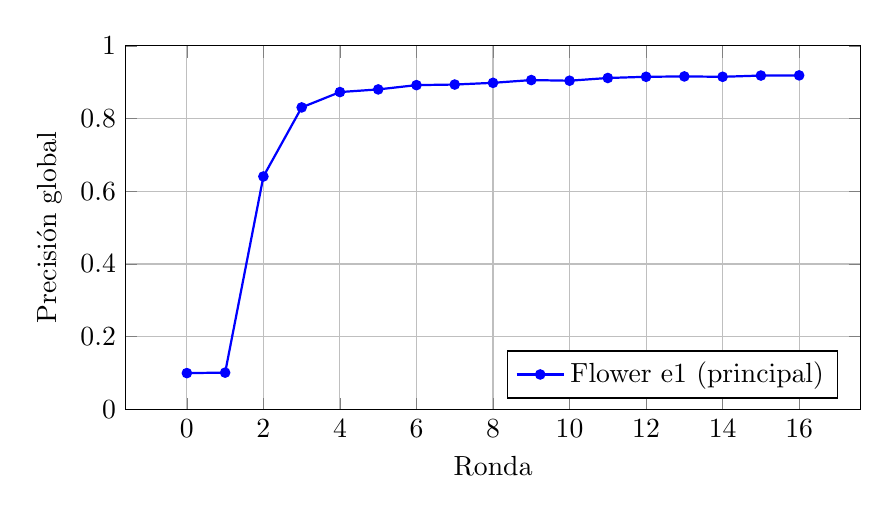
\begin{tikzpicture}
    \begin{axis}[width=0.9\textwidth, height=6.2cm,
      xlabel={Ronda}, ylabel={Precisión global}, ymin=0, ymax=1,
      grid=major, legend pos=south east, mark size=1.5pt]
      \addplot[blue, thick, mark=*] coordinates {
        (0,0.1000)(1,0.1013)(2,0.6407)(3,0.8306)(4,0.8728)(5,0.8801)(6,0.8919)
        (7,0.8935)(8,0.8982)(9,0.9058)(10,0.9040)(11,0.9115)(12,0.9148)(13,0.9158)
        (14,0.9148)(15,0.9182)(16,0.9187)};
      \addlegendentry{Flower e1 (principal)}
    \end{axis}
  \end{tikzpicture}
  \caption{Convergencia de la precisión global de Flower en el experimento principal (rondas
  registradas en los \textit{logs}).}
  \label{fig:flower-conv}
\end{figure}

En modo concurrente, Flower no produjo resultados comparables en el equipo utilizado. La
simulación concurrente lanza varios clientes en paralelo mediante Ray y, en repetidas
ejecuciones, el nodo superó el umbral de memoria configurado por Ray, que terminó procesos de
trabajo con el error \textit{OutOfMemoryError}. Como consecuencia, las rondas recibían menos
resultados de los esperados o la ejecución quedaba incompleta, con precisiones que no superaban
el comportamiento inicial. Estos resultados se tratan, por tanto, como una incidencia del
entorno y se retoman en la Sección~\ref{sec:concurrencia}.

\section{NVIDIA FLARE}\label{sec:resultados-nvflare}

La Tabla~\ref{tab:nvflare-seq} resume los resultados secuenciales de NVIDIA FLARE. La
configuración principal alcanza un 91{,}58\,\% de precisión, muy cerca de Flower, pero con el
tiempo de ejecución más alto del estudio (algo más de tres horas) y la utilización media de GPU
más elevada. El comportamiento en escalabilidad reproduce de nuevo la caída de precisión al
aumentar el número de clientes, y el experimento de participación parcial obtiene un buen
resultado (90{,}86\,\%) completando las veinte rondas.

\begin{table}[htbp]
  \centering
  \footnotesize
  \setlength{\tabcolsep}{4pt}
  \caption{Resultados de NVIDIA FLARE en modo secuencial. La RAM corresponde al proceso
  principal.}
  \label{tab:nvflare-seq}
  \begin{tabular}{lcccccccccc}
    \toprule
    Exp. & Cli. & Ron. & Acc. & Loss & Tiempo (s) & GPU (MiB) & Util. (\%) & Energía (Wh) & Temp. (\textdegree C) & RAM (GiB) \\
    \midrule
    e0    & 10 & 30 & 0,8260 & 0,5564 & 5758  & 466 & 56,90 & 51,76  & 83 & 2,2 \\
    e1    & 5  & 20 & 0,9158 & 0,2866 & 11074 & 466 & 91,33 & 131,15 & 87 & 2,1 \\
    e2-c4 & 4  & 10 & 0,8145 & 0,5796 & 1320  & 468 & 75,97 & 14,84  & 66 & 1,8 \\
    e2-c5 & 5  & 10 & 0,8167 & 0,5510 & 1404  & 466 & 71,06 & 15,08  & 66 & 1,8 \\
    e2-c8 & 8  & 10 & 0,7713 & 0,6605 & 1617  & 470 & 61,80 & 16,01  & 68 & 2,0 \\
    e3    & 8  & 20 & 0,9086 & 0,3277 & 5593  & 470 & 87,59 & 70,61  & 87 & 2,0 \\
    \bottomrule
  \end{tabular}
\end{table}

A diferencia de Flower, NVIDIA FLARE no realiza una evaluación centralizada del modelo global en
cada ronda, sino únicamente al final de la ejecución, por lo que no se dispone de una curva de
convergencia \emph{global} por ronda equivalente a la de la Figura~\ref{fig:flower-conv}. No
obstante, el simulador sí registra en cada ronda la validación local de los clientes, cuya media
permite trazar la evolución del entrenamiento. La Figura~\ref{fig:nvflare-conv} muestra esa
precisión de validación local media por ronda en el experimento principal: la convergencia es
rápida en las primeras rondas y se estabiliza en torno al 83--84\,\% a partir de la ronda diez.
Conviene subrayar que esta curva refleja la validación local sobre las particiones de cada
cliente, no la evaluación centralizada sobre el conjunto de prueba completo; por eso su valor
final (84{,}29\,\%) queda por debajo de la precisión centralizada final del modelo global
(91{,}58\,\%), medida sobre las 10\,000 imágenes de prueba.

\begin{figure}[htbp]
  \centering
  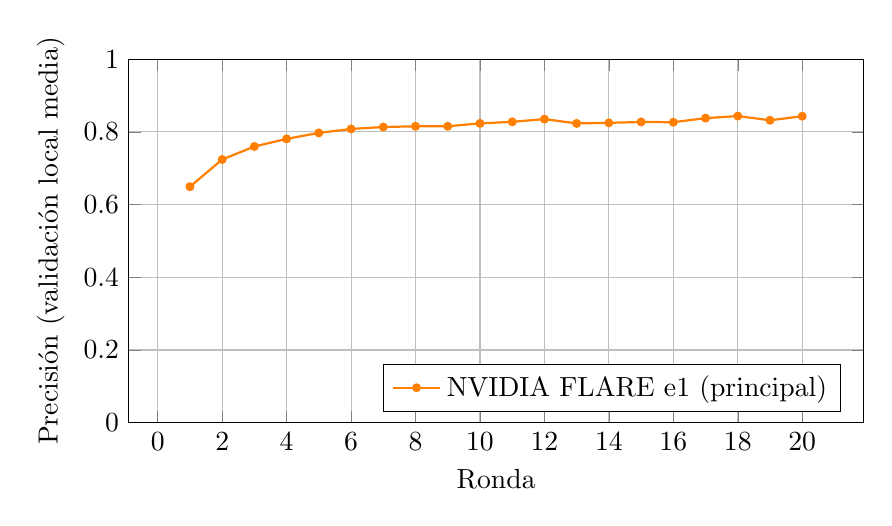
\begin{tikzpicture}
    \begin{axis}[width=0.9\textwidth, height=6.2cm,
      xlabel={Ronda}, ylabel={Precisión (validación local media)}, ymin=0, ymax=1,
      grid=major, legend pos=south east, mark size=1.2pt]
      \addplot[orange, thick, mark=*] coordinates {
        (1,0.6491)(2,0.7239)(3,0.7596)(4,0.7806)(5,0.7970)(6,0.8079)(7,0.8132)
        (8,0.8152)(9,0.8153)(10,0.8232)(11,0.8274)(12,0.8350)(13,0.8231)(14,0.8247)
        (15,0.8271)(16,0.8264)(17,0.8376)(18,0.8434)(19,0.8317)(20,0.8429)};
      \addlegendentry{NVIDIA FLARE e1 (principal)}
    \end{axis}
  \end{tikzpicture}
  \caption{Evolución por ronda de la precisión de validación local media de NVIDIA FLARE en el
  experimento principal. Se trata de la media de la validación local de los clientes en cada
  ronda, no de una evaluación centralizada del modelo global; la precisión centralizada final
  fue del 91{,}58\,\%.}
  \label{fig:nvflare-conv}
\end{figure}

En modo concurrente, NVIDIA FLARE tampoco proporcionó resultados utilizables. Al aumentar el
número de hilos de entrenamiento del simulador, crece el número de procesos y clientes activos
de forma simultánea, y en el equipo utilizado esto provocó cuelgues del sistema que obligaron a
reiniciar la máquina. No se afirma que se produjera un agotamiento de memoria de GPU, ya que no
se dispone de un registro que lo demuestre; lo observado es una saturación de memoria y procesos
del sistema. Estos casos se documentan en la Sección~\ref{sec:concurrencia}.

\section{FedML}\label{sec:resultados-fedml}

La Tabla~\ref{tab:fedml-seq} recoge los resultados secuenciales de FedML. El experimento de
referencia (e0) es el único con métricas de GPU fiables; en el resto de ejecuciones secuenciales
el muestreo de GPU falló por un problema de versión de NVML, de modo que esas columnas figuran
como no disponibles (N/D), aunque las métricas de aprendizaje, tiempo y memoria sí son válidas.
FedML reproduce la tendencia de escalabilidad de los otros dos \textit{frameworks}, con la
particularidad de una caída de precisión más acusada con ocho clientes (69{,}40\,\%).

\begin{table}[htbp]
  \centering
  \footnotesize
  \setlength{\tabcolsep}{4pt}
  \caption{Resultados de FedML en modo secuencial. Las métricas de GPU solo son fiables en e0
  (en el resto falló NVML). La RAM corresponde al proceso principal.}
  \label{tab:fedml-seq}
  \begin{tabular}{lccccccc}
    \toprule
    Exp. & Cli. & Ron. & Acc. & Loss & Tiempo (s) & GPU/Util./Energía & RAM (GiB) \\
    \midrule
    e0    & 10 & 30 & 0,8320 & 0,4981 & 3447 & 414 MiB / 95,23\,\% / 48,1 Wh & 2,6 \\
    e1    & 5  & 20 & 0,9086 & 0,4171 & 9647 & N/D & 2,3 \\
    e2-c4 & 4  & 10 & 0,7916 & 0,5912 & 1273 & N/D & 2,2 \\
    e2-c5 & 5  & 10 & 0,7689 & 0,6510 & 1293 & N/D & 2,3 \\
    e2-c8 & 8  & 10 & 0,6940 & 0,8508 & 1232 & N/D & 2,4 \\
    e3    & 8  & 20 & 0,8835 & 0,4604 & 5287 & N/D & 2,2 \\
    \bottomrule
  \end{tabular}
\end{table}

FedML registra la precisión de prueba en cada ronda de comunicación, lo que permite trazar la
curva de convergencia completa del experimento de referencia (Figura~\ref{fig:fedml-conv}). La
curva muestra una mejora sostenida a lo largo de las treinta rondas, sin la estabilización
temprana observada en Flower, coherente con una configuración de solo dos épocas locales por
ronda que avanza de forma más gradual.

\begin{figure}[htbp]
  \centering
  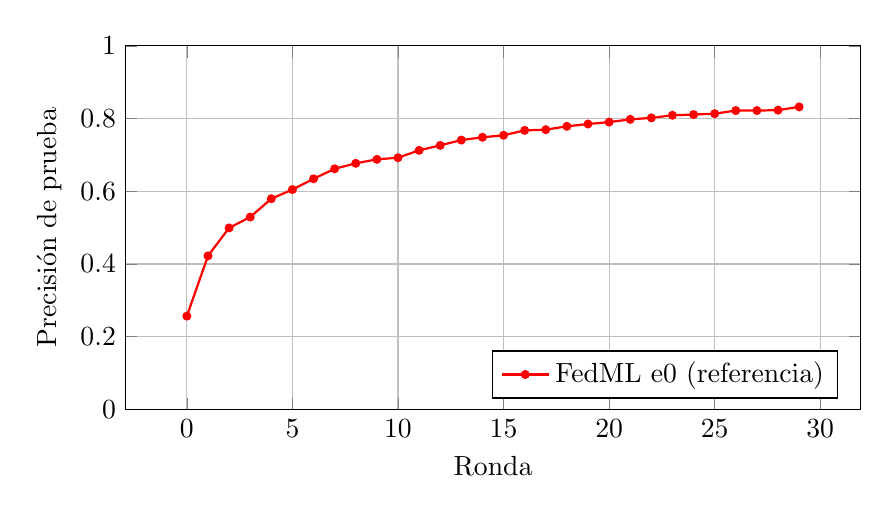
\begin{tikzpicture}
    \begin{axis}[width=0.9\textwidth, height=6.2cm,
      xlabel={Ronda}, ylabel={Precisión de prueba}, ymin=0, ymax=1,
      grid=major, legend pos=south east, mark size=1.2pt]
      \addplot[red, thick, mark=*] coordinates {
        (0,0.2567)(1,0.4224)(2,0.4992)(3,0.5291)(4,0.5795)(5,0.6047)(6,0.6343)
        (7,0.6618)(8,0.6769)(9,0.6878)(10,0.6923)(11,0.7125)(12,0.7262)(13,0.7408)
        (14,0.7484)(15,0.7540)(16,0.7674)(17,0.7694)(18,0.7786)(19,0.7850)(20,0.7902)
        (21,0.7977)(22,0.8018)(23,0.8090)(24,0.8109)(25,0.8134)(26,0.8219)(27,0.8219)
        (28,0.8231)(29,0.8320)};
      \addlegendentry{FedML e0 (referencia)}
    \end{axis}
  \end{tikzpicture}
  \caption{Convergencia de la precisión de prueba de FedML en el experimento de referencia
  (treinta rondas completas).}
  \label{fig:fedml-conv}
\end{figure}

A diferencia de los otros dos \textit{frameworks}, el modo concurrente de FedML sí se ejecutó.
El backend MPI, lanzado con \texttt{mpirun}, mantiene varios procesos de cliente en paralelo y
completó las ejecuciones registrando métricas de tiempo y de consumo de recursos
(Tabla~\ref{tab:fedml-conc}). Sin embargo, estas ejecuciones no guardaron una precisión final
extraíble en los \textit{logs} analizados, por lo que se utilizan únicamente para describir el
comportamiento computacional del modo concurrente, no para comparar la calidad del modelo. Se
observa una utilización de GPU muy alta (cercana al 100\,\%) y un uso de memoria de GPU
sensiblemente mayor que en secuencial, que crece con el número de clientes.

\begin{table}[htbp]
  \centering
  \footnotesize
  \setlength{\tabcolsep}{4pt}
  \caption{Resultados de FedML en modo concurrente (backend MPI). No se dispone de precisión
  final extraída; solo se reportan tiempo y consumo de recursos.}
  \label{tab:fedml-conc}
  \begin{tabular}{lcccccccc}
    \toprule
    Exp. & Cli. & Ron. & Tiempo (s) & GPU (MiB) & Util. (\%) & Pot. media (W) & Temp. (\textdegree C) & RAM (GiB) \\
    \midrule
    e1    & 5 & 20 & 11380 & 2358 & 99,80 & 43,15 & 80 & 2,0 \\
    e2-c4 & 4 & 10 & 1102  & 1907 & 98,91 & 46,01 & 80 & 2,1 \\
    e2-c5 & 5 & 10 & 1109  & 2358 & 98,81 & 49,60 & 87 & 2,0 \\
    e2-c8 & 8 & 10 & 1114  & 3727 & 97,84 & 50,61 & 85 & 1,8 \\
    e3    & 8 & 20 & 5457  & 1915 & 99,61 & 49,45 & 83 & 2,1 \\
    \bottomrule
  \end{tabular}
\end{table}

\section{Comparativa entre frameworks}\label{sec:comparativa-frameworks}

Esta sección compara los tres \textit{frameworks} sobre las métricas comunes del modo secuencial,
que es el que ofrece resultados de aprendizaje equiparables.

\subsection{Precisión final}\label{sec:comp-precision}

La Figura~\ref{fig:comp-acc} compara la precisión final por experimento. En el experimento
principal (e1) los tres \textit{frameworks} quedan muy próximos, encabezados por Flower
(92{,}03\,\%), seguido de NVIDIA FLARE (91{,}58\,\%) y FedML (90{,}86\,\%). Las diferencias son
mayores en los experimentos de menor duración: en escalabilidad, FedML obtiene precisiones algo
inferiores, especialmente con ocho clientes. En participación parcial (e3), NVIDIA FLARE y FedML
superan claramente a Flower, cuyo resultado en ese experimento debe tomarse con cautela por su
seguimiento incompleto.

\begin{figure}[htbp]
  \centering
  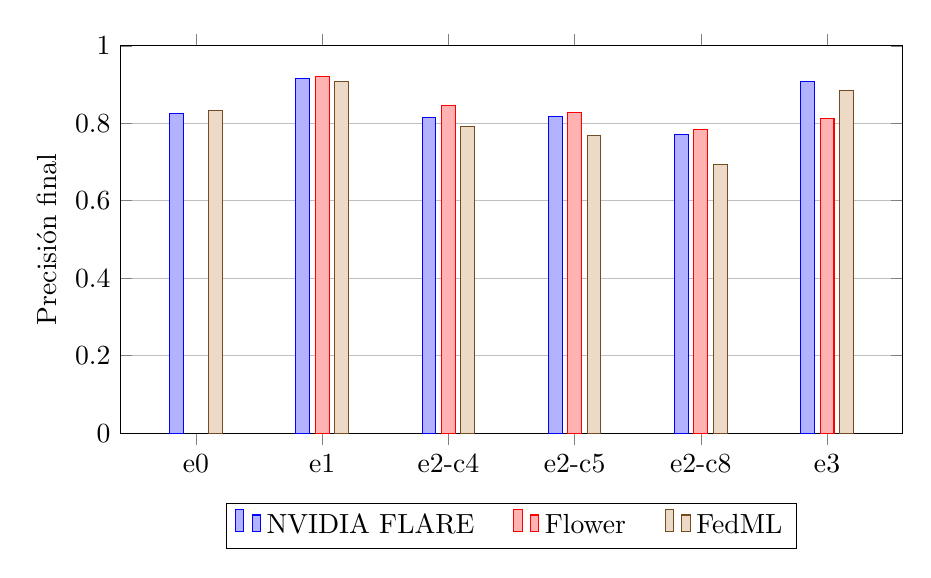
\begin{tikzpicture}
    \begin{axis}[ybar, bar width=5pt, width=0.95\textwidth, height=6.5cm,
      symbolic x coords={e0,e1,e2-c4,e2-c5,e2-c8,e3}, xtick=data,
      ymin=0, ymax=1, ylabel={Precisión final},
      legend style={at={(0.5,-0.18)}, anchor=north, legend columns=-1,
        /tikz/every even column/.append style={column sep=12pt}},
      enlarge x limits=0.12, ymajorgrids]
      \addplot coordinates {(e0,0.8260)(e1,0.9158)(e2-c4,0.8145)(e2-c5,0.8167)(e2-c8,0.7713)(e3,0.9086)};
      \addplot coordinates {(e1,0.9203)(e2-c4,0.8451)(e2-c5,0.8277)(e2-c8,0.7839)(e3,0.8119)};
      \addplot coordinates {(e0,0.8320)(e1,0.9086)(e2-c4,0.7916)(e2-c5,0.7689)(e2-c8,0.6940)(e3,0.8835)};
      \legend{NVIDIA FLARE, Flower, FedML}
    \end{axis}
  \end{tikzpicture}
  \caption{Precisión final por experimento y \textit{framework} (modo secuencial). Flower no
  dispone de experimento de referencia válido.}
  \label{fig:comp-acc}
\end{figure}

\subsection{Tiempo de ejecución}\label{sec:comp-tiempo}

La Figura~\ref{fig:comp-tiempo} compara la duración. Los experimentos con muchas épocas locales
(e1 y e3) dominan el tiempo total, como era de esperar. En el experimento principal, FedML es el
más rápido (unas 2,7 horas), seguido de Flower (3,3 horas) y NVIDIA FLARE (3,1 horas). En los
experimentos cortos de escalabilidad los tres \textit{frameworks} quedan en el mismo orden de
magnitud, en torno a veinte minutos.

\begin{figure}[htbp]
  \centering
  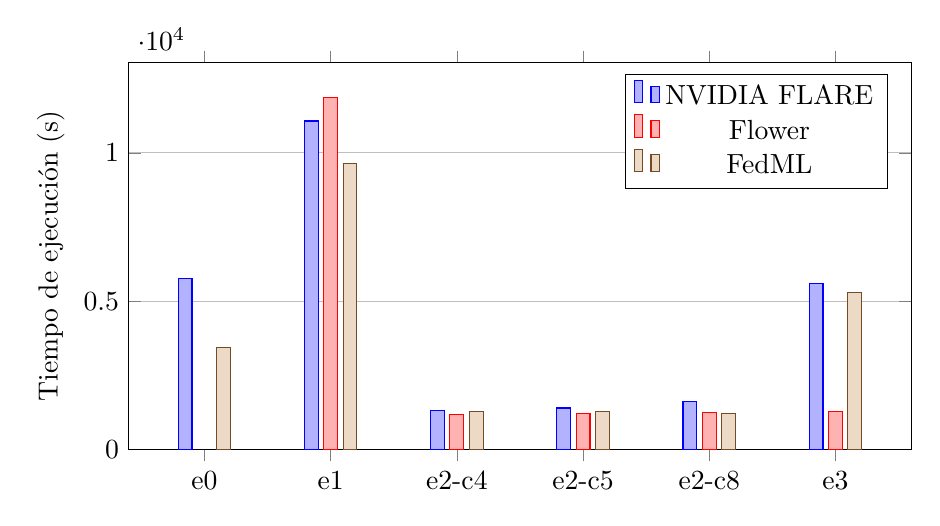
\begin{tikzpicture}
    \begin{axis}[ybar, bar width=5pt, width=0.95\textwidth, height=6.5cm,
      symbolic x coords={e0,e1,e2-c4,e2-c5,e2-c8,e3}, xtick=data,
      ymin=0, ylabel={Tiempo de ejecución (s)}, legend pos=north east,
      enlarge x limits=0.12, ymajorgrids]
      \addplot coordinates {(e0,5758)(e1,11074)(e2-c4,1320)(e2-c5,1404)(e2-c8,1617)(e3,5593)};
      \addplot coordinates {(e1,11864)(e2-c4,1196)(e2-c5,1216)(e2-c8,1240)(e3,1290)};
      \addplot coordinates {(e0,3447)(e1,9647)(e2-c4,1273)(e2-c5,1293)(e2-c8,1232)(e3,5287)};
      \legend{NVIDIA FLARE, Flower, FedML}
    \end{axis}
  \end{tikzpicture}
  \caption{Tiempo de ejecución por experimento y \textit{framework} (modo secuencial). El valor
  de Flower en e3 corresponde a una ejecución con seguimiento incompleto.}
  \label{fig:comp-tiempo}
\end{figure}

\subsection{Escalabilidad}\label{sec:comp-escalabilidad}

La Figura~\ref{fig:comp-escala} muestra la precisión final frente al número de clientes en los
experimentos de escalabilidad (cuatro, cinco y ocho clientes, con dos épocas locales y diez
rondas). Los tres \textit{frameworks} pierden precisión a medida que aumenta el número de
clientes, lo que es coherente con el reparto del conjunto: con más clientes, cada uno entrena con
menos datos y el mismo número de rondas resulta insuficiente para alcanzar la misma calidad. La
pendiente es más pronunciada en FedML.

\begin{figure}[htbp]
  \centering
  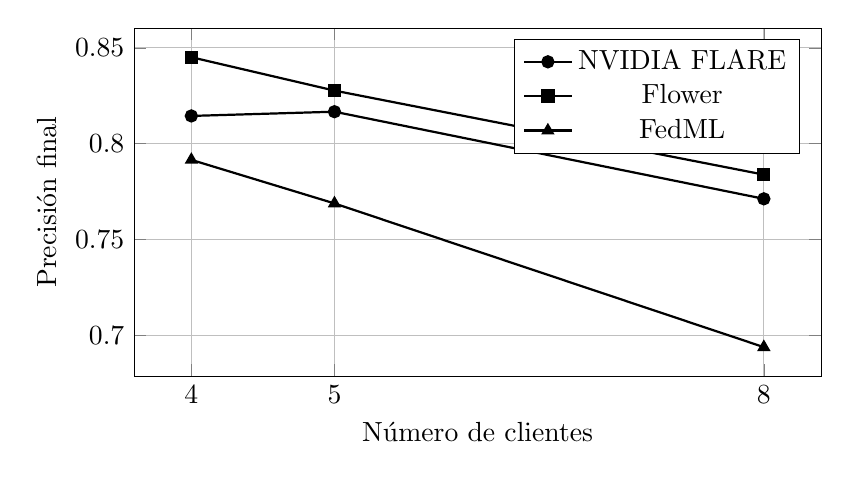
\begin{tikzpicture}
    \begin{axis}[width=0.85\textwidth, height=6cm,
      xlabel={Número de clientes}, ylabel={Precisión final},
      xtick={4,5,8}, grid=major, legend pos=north east, mark size=2pt]
      \addplot[thick, mark=*]      coordinates {(4,0.8145)(5,0.8167)(8,0.7713)};
      \addplot[thick, mark=square*] coordinates {(4,0.8451)(5,0.8277)(8,0.7839)};
      \addplot[thick, mark=triangle*] coordinates {(4,0.7916)(5,0.7689)(8,0.6940)};
      \legend{NVIDIA FLARE, Flower, FedML}
    \end{axis}
  \end{tikzpicture}
  \caption{Precisión final frente al número de clientes en los experimentos de escalabilidad
  (modo secuencial).}
  \label{fig:comp-escala}
\end{figure}

\subsection{Consumo de recursos}\label{sec:comp-recursos}

La Figura~\ref{fig:comp-energia} compara la energía estimada de los tres \textit{frameworks}. De
FedML solo se incluye el experimento de referencia (e0), el único con métricas de GPU fiables, ya
que en el resto de sus ejecuciones secuenciales falló el muestreo por el problema de NVML; su
valor en e0 (en torno a 48\,Wh) es muy próximo al de NVIDIA FLARE (51{,}76\,Wh) en esa misma
configuración. El consumo energético sigue de cerca al tiempo de ejecución y a la utilización de
GPU: los experimentos largos con muchas épocas locales (e1 y e3) concentran el mayor gasto. En el
experimento principal Flower y NVIDIA FLARE consumen una energía similar (en torno a
130--137\,Wh), mientras que NVIDIA FLARE presenta un consumo notablemente mayor en participación
parcial, asociado a su mayor tiempo de ejecución en ese caso.

\begin{figure}[htbp]
  \centering
  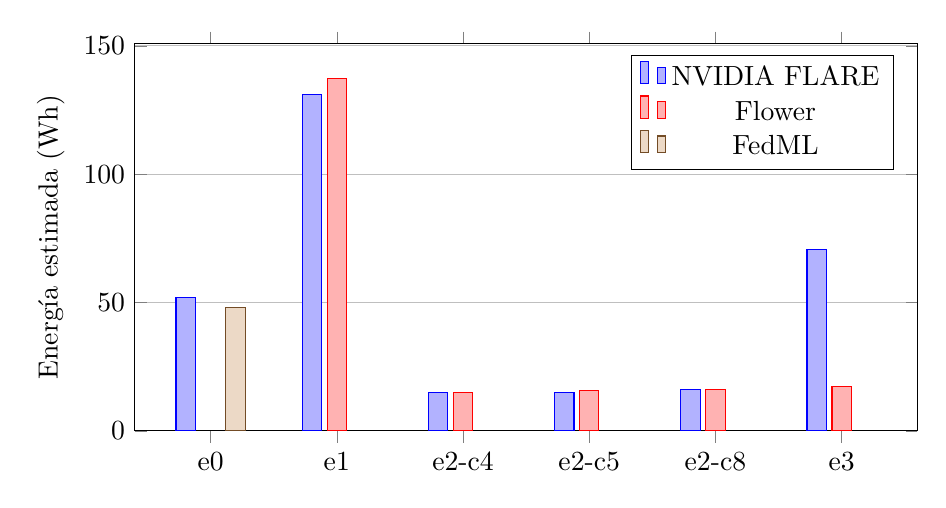
\begin{tikzpicture}
    \begin{axis}[ybar, bar width=7pt, width=0.95\textwidth, height=6.5cm,
      symbolic x coords={e0,e1,e2-c4,e2-c5,e2-c8,e3}, xtick=data,
      ymin=0, ylabel={Energía estimada (Wh)}, legend pos=north east,
      enlarge x limits=0.12, ymajorgrids]
      \addplot coordinates {(e0,51.76)(e1,131.15)(e2-c4,14.84)(e2-c5,15.08)(e2-c8,16.01)(e3,70.61)};
      \addplot coordinates {(e1,137.18)(e2-c4,14.92)(e2-c5,15.57)(e2-c8,16.02)(e3,17.16)};
      \addplot coordinates {(e0,48.10)};
      \legend{NVIDIA FLARE, Flower, FedML}
    \end{axis}
  \end{tikzpicture}
  \caption{Energía estimada por experimento (modo secuencial). De FedML solo se dispone del
  experimento de referencia (e0), por el fallo de NVML en el resto de sus ejecuciones.}
  \label{fig:comp-energia}
\end{figure}

En cuanto a la memoria de GPU, los tres \textit{frameworks} se mantienen muy por debajo de los
6\,GB disponibles en el modo secuencial: NVIDIA FLARE en torno a 466\,MiB, Flower alrededor de
760\,MiB y FedML unos 414\,MiB en el experimento de referencia. La diferencia más relevante
aparece en el modo concurrente de FedML, donde la memoria de GPU crece de forma marcada con el
número de clientes (hasta 3727\,MiB con ocho clientes), lo que ilustra el coste del paralelismo
real entre procesos.

\subsection{Comportamiento en modo concurrente}\label{sec:concurrencia}

El modo concurrente puso de manifiesto las diferencias de arquitectura entre los tres
\textit{frameworks} y los límites del equipo utilizado. Cada herramienta implementa la
concurrencia de una forma distinta. Flower simula varios clientes en paralelo mediante Ray, que
lanza un actor por cliente dentro del mismo nodo. NVIDIA FLARE controla la concurrencia con el
número de hilos de entrenamiento del simulador, lo que se traduce en más procesos y clientes
activos a la vez. FedML, en su backend concurrente, recurre a MPI: \texttt{mpirun} arranca un
proceso independiente por cliente más uno de coordinación, que se comunican mediante paso de
mensajes.

El resultado en el equipo de pruebas, con 6\,GB de GPU y 14\,GiB de RAM, fue desigual. En Flower,
Ray terminó procesos de trabajo al superar el umbral de memoria del nodo, con errores explícitos
de \textit{OutOfMemoryError}; los ajustes probados, como reducir el número de procesos de carga
de datos o liberar la caché, no evitaron el fallo. En NVIDIA FLARE, el aumento de hilos provocó
una saturación de memoria y procesos que llegó a colgar el sistema. FedML con MPI fue el único
que completó la ejecución concurrente, a costa de una utilización de GPU cercana al 100\,\% y de
un mayor consumo de memoria de GPU, aunque sin proporcionar una precisión final extraíble en los
\textit{logs}: en el \textit{backend} MPI las ejecuciones finalizaron sin registrar una
evaluación final comparable, de modo que solo permiten analizar el comportamiento computacional.
Esa precisión podría recuperarse evaluando a posteriori el modelo final guardado con el mismo
procedimiento de evaluación centralizada usado en el modo secuencial, lo que queda planteado como
trabajo futuro. En conjunto, ningún \textit{framework} resultó inmune a las limitaciones de
recursos en modo concurrente, si bien solo FedML representó una concurrencia real entre procesos.

\section{Síntesis}\label{sec:sintesis-resultados}

En modo secuencial los tres \textit{frameworks} alcanzan precisiones muy similares en el
experimento principal, lo que confirma que, bajo idénticas condiciones de datos, modelo e
hiperparámetros, la elección de la herramienta influye poco en la calidad del modelo y mucho en
el coste de obtenerlo. Las diferencias más claras aparecen en el tiempo de ejecución, en la
utilización de GPU y, sobre todo, en la estabilidad del modo concurrente, donde el equipo
utilizado marcó el límite. Estos resultados cuantitativos se complementan con la valoración
cualitativa de usabilidad y flexibilidad del capítulo siguiente, que ayuda a interpretar cuándo
conviene cada \textit{framework} más allá de las cifras de rendimiento.
